\chapter*{Secondary Contributions}
\addcontentsline{toc}{chapter}{Secondary Contributions}
\label{Secondary_Contributions}

\textbf{PET FDG Improved Tumour Definition using Deep Learning}

Within the \gls{hybrid} secondments schedule, a 1-month secondment for Laura Dal Toso (LDT) from King's College London (KCL) was planned to take place at our lab. This secondment aimed in performing simulations for creation of large datasets that could be used for the training of Deep Learning (DL) methods.

For applications of PET imaging in oncology, quantification and shape of tumours are regularly used by medical professionals for the characterisation and classification of disease. For the case of \gls{nsclc} imaging, and not only limited to that, these image characteristics are often degraded by image noise and partial volume effects.
In this work, a method for improving tumour shape definition and quantification was proposed, by use of Deep Learning (DL). As DL methods require a large number of training datasets, simulations were used to train the proposed DL method. 

The aim was to ultimately use the DL method for real \gls{nsclc} image data from an mMR PET/MR scanner (installed at KCL). Thus the implementation of the mMR geometry in the PET analytical simulator was needed, which was performed by me (ZC) with guidance from Dr Simon Stute. After the successful integration of the geometry for simulations and validation of reconstructions using CASToR, a large dataset of ground truth tumours (placed within the XCAT phantom) was created by LDT and provided for PET simulation. A total of 2210 cases were simulated and reconstructed, using a custom made pipeline by ZC on two computer clusters of our lab.
Details on the methodology used and results are provided in the attached draft paper, which will be submitted for publication.

\textbf{Data Driven Motion Correction for Brain PET Dynamic Imaging}

A 2-week secondment was planned for me at the MUW in Vienna, with the aim of making use of dynamic reconstruction techniques developed during this PhD project to a cohort of epilepsy dynamic PET data. But this secondment was performed mostly from distance due to the pandemic and the time was spent towards the implementation and evaluation of novel motion estimation method for dynamic PET brain studies. 

Towards this goal, a method was developed using ultra-short frame reconstruction 
and a Cycle Generative Adversarial Network (cGAN). The cGAN was designed to improve image quality of the short frame reconstructions for better motion estimation. In the training of the cGAN, data from the cohort of epilepsy patients was used. The datasets had been acquired on an mMR PET/MR scanner.

During this project, a converter was adapted to support conversion of dynamic mMR PET data, including all corrections generated by the e7 tools, to the CASToR datafile format. Using the converted data, dynamic reconstructions were performed in CASToR using the involuntary motion correction option. These reconstructions were used to assess the effect of intra-frame motion correction in result activity and parametric images.
The development work and application of the cGAN has resulted in the attached publication by Shiyam Sundar \textit{et al.}~\cite{ShiyamSundar2020}. The work performed using CASToR has not been included in this publication, but it is considered for use in a future project on the topic of motion correction.

\cleardoublepage
\includepdf[pages=-]{SecondaryContributions/Formatted_Paper.pdf}
\cleardoublepage
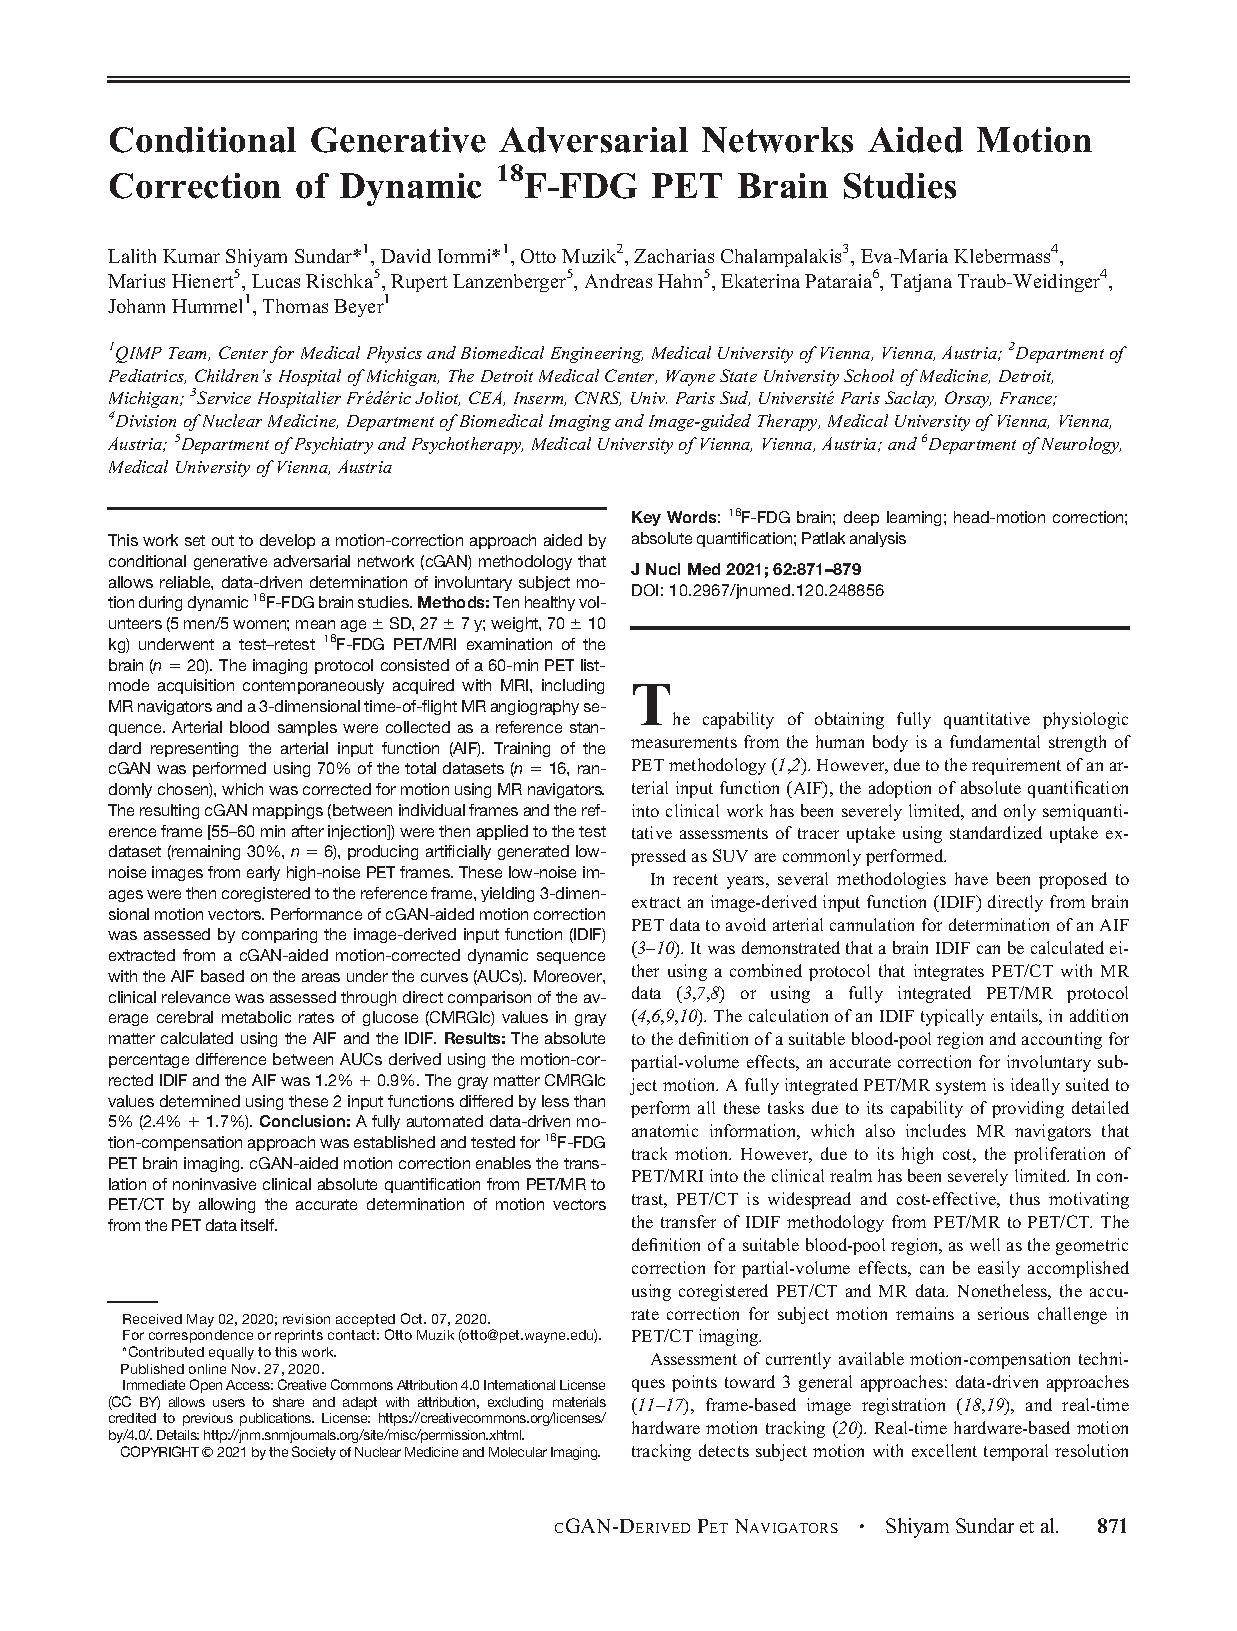
\includepdf[pages=-]{SecondaryContributions/871.full.pdf}